% 多区间二分法

\pentry{二分法\upref{Bisec}}

这里介绍一种多区间二分法, 可以求出连续函数在某区间内几乎全部的根. 方法就是把这个区间等分为若干个相等的小区间, 然后分别判断这些小区间两端函数值的符号, 对所有两端异号的区间使用二分法即可. 显然, 小区间的个数越多, 越有可能找到所有的根. 例程如下.

\subsubsection{bisectionN.m}
\Matlab
function roots = bisectionN(f, int, N)
x = linspace(int(1), int(2), N); % 划分区间
y = arrayfun(f, x); % 求所有 f(x(ii))
figure; plot(x, y, '.-') % 画图
title('f(x)')
Sign = sign(y);
ind = find(Sign(1:end-1) .* Sign(2:end) <= 0); % 找符合条件的区间序号
Nroot = numel(ind);
roots = zeros(1, Nroot); % 预赋值
for ii = 1:Nroot
    roots(ii) = fzero(f, [x(ind(ii)),x(ind(ii)+1)]);  
end
end
\end{lstlisting}

函数的前两个输入变量分别是需要求根的函数句柄和求根区间(二元行矢量或列矢量), 第三个变量 $N$ 是子区间端点的个数(即子区间的个数加一). 函数中先求出所有的端点 \x{x}, 以及对应的函数值 \x{y}, 然后画图. 第 6-7 行寻找所有两端异号或有一端为 0 的区间的序号, 然后在第 10 行的循环中对这些区间逐个使用二分法. 为了提高运算效率, 这里并没有使用“二分法\upref{Bisec}” 中的例程, 而是使用了 Matlab 自带的 \x{fzero} 函数.

\x{bisectionN} 的画图功能是为了让用户判断是否有可能出现漏根, 以下举两个例子说明.
\begin{Command}
>> f = @(x)exp(-0.2*x)*sin(x); \\
>> roots = bisectionN(f, [0, 15], 50)\\
roots = 0    3.1416    6.2832    9.4248   12.5664
\end{Command}
\begin{figure}[ht]
\centering
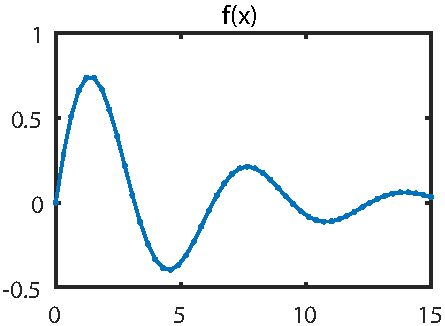
\includegraphics[width=8cm]{./figures/MBisec.pdf}
\caption{运行结果} \label{MBisec_fig1}
\end{figure}
运行结果如\autoref{MBisec_fig1}, 由于画出的曲线较为光滑, 可判断漏根的可能性很小. 再看另一个例子
\begin{Command}
>> f = @(x)sin(1/x); \\
>> roots = bisectionN(f, [0, 0.3], 50)\\
roots = 0.0245    0.0398    0.0455    0.0531    0.0637    0.0796    0.1061    0.1592
\end{Command}
\begin{figure}[ht]
\centering
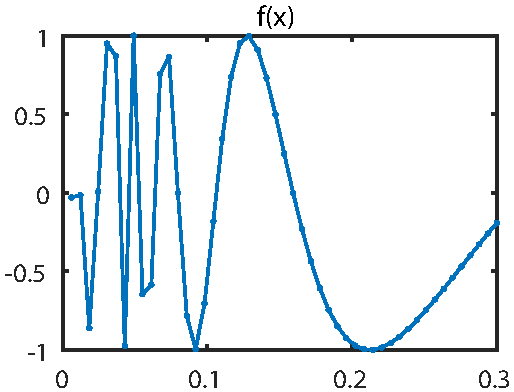
\includegraphics[width=8cm]{./figures/MBisec2.pdf}
\caption{运行结果} \label{MBisec_fig2}
\end{figure}
我们已经知道函数 $\sin(1/x)$ 在该区间上有无数个根, 且越接近 $x = 0$, 相邻根之间的距离越小. 运行结果如\autoref{MBisec_fig2},  可见在区间 $[0, 0.1]$ 内, 子区间端点的函数值非常不平滑, 极有可能出现漏根. 为了求得更多的根, 我们可以增加子区间的个数.
